
\section{Potence in izrazi}

\begin{frame}
    \sectionpage
\end{frame}

\begin{frame}
    \tableofcontents[currentsection, hideothersubsections]
\end{frame}

\subsection{Potence z naravnim eksponentom}


\begin{frame}
    \frametitle{Potence z naravnim eksponentom}

    \only<2->{\begin{alertblock}{Potenca z naravnim eksponentom}
        Potenca $\mathbf{x^n}$ z \textbf{osnovo}/\textbf{bazo} $x$ in \textbf{eksponentom}/\textbf{stopnjo} $n \in \mathbb{N}$, je produkt $n$ faktorjev enakih $x$.

        \only<3->{$$ \mathbf{x^n=\underbrace{x\cdot x\cdot \ldots \cdot x}_\text{n faktorjev}}  $$}
    \end{alertblock}}
    
    \only<4->{\begin{block}{}
        \begin{figure}
            \begin{tikzpicture}

                \draw[thick] (0,0)--(2,0); 
                \node at (1,0.15) {$x$};

                \only<5->{\fill[red!40] (3,0) rectangle (5,2);
                \draw[black,thick] (3,0) rectangle (5,2); 
                \node at (4,1) {$x^2$};}

                \only<6->{\fill[red!40] (6,0) rectangle (8,2);
                \fill[red!40] (7,2.5)--(6,2)--(8,2)--(9,2.5)--cycle;
                \fill[red!40] (8,0)--(9,0.5)--(9,2.5)--(8,2)--cycle;
                \draw[black,thick] (6,0) rectangle (8,2);
                \draw[black,thick] (7,2.5)--(6,2)--(8,2)--(9,2.5)--cycle;
                \draw[black,thick] (8,0)--(9,0.5)--(9,2.5)--(8,2)--cycle;
                \node at (7,1) {$x^3$};}
            
            \end{tikzpicture}
        \end{figure}
    \end{block}}

\end{frame}

\subsection{Pravila za računanje s potencami}
\begin{frame}
    \frametitle{Pravila za računanje s potencami}
    
    \only<2->{\begin{block}{}
        \only<2>{$$ x^n \cdot x^m=$$}
        \only<3>{$$ x^n \cdot x^m=\underbrace{(x\cdot x\cdot\ldots\cdot x)}_\text{n faktorjev}\cdot\underbrace{(x\cdot x\cdot\ldots\cdot x)}_\text{m faktorjev}=$$}
        \only<4->{$$ x^n \cdot x^m=\underbrace{(x\cdot x\cdot\ldots\cdot x)}_\text{n faktorjev}\cdot\underbrace{(x\cdot x\cdot\ldots\cdot x)}_\text{m faktorjev}=x^{n+m}$$}

        

        \only<5->{Dve potenci z isto osnovo zmnožimo tako, da osnovo ohranimo, eksponenta pa seštejemo.}
    \end{block}}

    \only<6->{\begin{block}{}
        \only<6>{$$ (x^n)^m=$$}
        \only<7>{$$ (x^n)^m=\underbrace{\underbrace{(x\cdot x\cdot\ldots\cdot x)}_\text{n faktorjev}\cdot\underbrace{(x\cdot x\cdot\ldots\cdot x)}_\text{n faktorjev}\cdot\ldots\cdot\underbrace{(x\cdot x\cdot\ldots\cdot x)}_\text{n faktorjev}}_\text{m faktorjev}=$$}
        \only<8->{$$ (x^n)^m=\underbrace{\underbrace{(x\cdot x\cdot\ldots\cdot x)}_\text{n faktorjev}\cdot\underbrace{(x\cdot x\cdot\ldots\cdot x)}_\text{n faktorjev}\cdot\ldots\cdot\underbrace{(x\cdot x\cdot\ldots\cdot x)}_\text{n faktorjev}}_\text{m faktorjev}=x^{n\cdot m}$$}
        
        \only<9->{Potenco potenciramo tako, da osnovo ohranimo, ekponenta pa zmnožimo.}
    \end{block}}

\end{frame}

\begin{frame}

    \only<2->{\begin{block}{}
        \only<2>{$$ (xy)^n =$$}
        \only<3>{$$ (xy)^n =\underbrace{(xy\cdot xy\cdot\ldots\cdot xy)}_\text{n faktorjev}=\underbrace{(x\cdot x\cdot\ldots\cdot x)}_\text{n faktorjev}\cdot\underbrace{(y\cdot y\cdot\ldots\cdot y)}_\text{n faktorjev}=$$}
        \only<4->{$$ (xy)^n =\underbrace{(xy\cdot xy\cdot\ldots\cdot xy)}_\text{n faktorjev}=\underbrace{(x\cdot x\cdot\ldots\cdot x)}_\text{n faktorjev}\cdot\underbrace{(y\cdot y\cdot\ldots\cdot y)}_\text{n faktorjev}=x^n y^n$$}



        \only<5->{Produkt dveh ali več števil potenciramo tako, da potenciramo posamezne faktorje in jih potem zmnožimo.}
    \end{block}}

    \only<6->{\begin{block}{}
        Za naravne eksponente velja še:
        \only<7->{$$(-x)^{2n}=x^{2n}$$}
        \only<8->{$$(-x)^{2n+1}=-x^{2n+1}$$}
    \end{block}}

    \only<9->{\begin{block}{}
        $$(-1)^n=\begin{cases}
            1; &n=2k \\
            -1; &n=2k-1
        \end{cases}; k\in\mathbb{N}$$
    \end{block}}
\end{frame}

\begin{frame}

    \only<2->{\begin{exampleblock}{Naloga}
        Števila $-3^2$, $(-4)^2$, $-2^4$, $(-1)^{2024}$, $(-2)^3$ in $(-3)^2$ uredite po velikosti od najmanjšega do največjega. \\ ~ \\ ~
    \end{exampleblock}}

    \only<3->{\begin{exampleblock}{Naloga}
        Poiščite podatke in jih zapišite na dva načina: s potenco in številom brez potence.
        \begin{itemize}
            \item Razdalja med Zemljo in Soncem
            \item Zemljina masa
            \item Masa Sonca
            \item Število zvezd v naši Galaksiji
        \end{itemize}
    \end{exampleblock}}

\end{frame}

\begin{frame}

    \only<2->{\begin{exampleblock}{Naloga}
        Izračunajte.
        \only<3->{\begin{itemize}
            \item $(-3)^2+2^4$ \\ ~
            \item $(5-3)^3+(-3)^2$ \\ ~
            \item $(2^2+1)^2+(-3)^3+(-2)^4$ \\ ~
            \item $(-1)^{2024}+((-2)^5+5^2-(7-3^2)^3)^2$ \\ ~
            \item $-1^{2n-1}+(-1)^{2n-1}$ \\ ~
        \end{itemize}}
    \end{exampleblock}}
\end{frame}

\begin{frame}
    \only<2->{\begin{exampleblock}{Naloga}
        Poenostavite izraz.
        \only<3->{\begin{itemize}
            \item $2^7\cdot 2^3$ \\~
            \item $a^3\cdot a^{12}\cdot a^5$ \\~
            \item $(2z)^3$ \\~
            \item $(m^2\cdot m^4)^3$ \\~
            \item $a^3+2a^3-6a^3$ \\~
            \item $x^2\cdot x^4+(-2x^3)^2-2(-x)^6$ \\~
        \end{itemize}}
    \end{exampleblock}}

\end{frame}


\begin{frame}
\only<2->{\begin{exampleblock}{Naloga}
    Izračunajte, rezultat zapišite s potenco.
    \only<3->{\begin{itemize}
        \item $2\cdot 10^3\cdot 3\cdot 10^2\cdot 5\cdot 10^6$ \\~
        \item $(10^3)^2\cdot5\cdot 10^4\cdot 2\cdot 10^3$ \\~
        \item $(-2)^3\cdot 2^7$ \\~
        \item $-2^3\cdot (-2)^4\cdot 2^3$ \\~
        \item $2^3\cdot(-3)^2\cdot 6^4\cdot 3$ \\~
        \item $(-3)^3\cdot(-7)^2\cdot 21^7\cdot 7$ \\~
    \end{itemize}}
\end{exampleblock}}
\end{frame}

\begin{frame}
\only<2->{\begin{exampleblock}{Naloga}
    Poenostavite.
    \only<3->{\begin{itemize}
        \item $2^3\cdot 3^4\cdot(2^4\cdot 3^2)^5$ \\~
        \item $(5^2\cdot 7)^3\cdot 5^2\cdot 7^3$ \\~
        \item $(-2^3\cdot 3^5)^4\cdot 2^6\cdot 3^5$ \\~
        \item $(-4)^2\cdot(-7)^{13}\cdot (-28)^5\cdot (-7^2)^3$ \\~
        \item $-6^2\cdot(-3)^2\cdot 8^5\cdot (-3^2)^3$ \\~
    \end{itemize}}
\end{exampleblock}}
\end{frame}

\begin{frame}
\only<2->{\begin{exampleblock}{Naloga}
    Poenostavite.
    \only<3->{\begin{itemize}
        \item $a^3\cdot b^2\cdot a^7\cdot b^3\cdot b^5$ \\~
        \item $4x^4\cdot(2x^3)^2$ \\~
        \item $(k^3\cdot 2h^5)^2$ \\~
        \item $(x^2y^4)^2\cdot (x^3y)^3$ \\~
        \item $(a^2b^5)^3(ab^3)^2$ \\~
        \item $x^2y^3(x^3y^6)^2$ \\~
    \end{itemize}}
\end{exampleblock}}
\end{frame}


\begin{frame}
\only<2->{\begin{exampleblock}{Naloga}
    Poenostavite.
    \only<3->{\begin{itemize}
        \item $2^3\cdot x^2\cdot 3^2\cdot(-x)^6$ \\~
        \item $(-a^3b)^4(-a^2b^5a^3)^3$ \\~
        \item $(2s^2\cdot(-s^2)^5)^5$ \\~
        \item $(-2(z^4)^2(-2z)^3z^5)^3$ \\~
        \item $(-3ab^2)^3(-a^4b^2(a^3)^5)^2(ab^3)^2$ \\~
        \item $(xy^2z)^3(x^3(-y^2)^5(-z))^3(x^2y^3(-z^2)^3)$ \\~
    \end{itemize}}
\end{exampleblock}}
\end{frame}

\begin{frame}
\only<2->{\begin{exampleblock}{Naloga}
    Odpravite oklepaje in poenostavite, če je mogoče.
    \only<3->{\begin{itemize}
        \item $a^n\cdot a^{n+2}\cdot(-a)^3$ \\ ~\\~
        \item $(-x^n)^4\cdot x^2$ \\~\\~
        \item $a^n\cdot(a^2-a^3+2)$ \\~\\~
        \item $(x^2+3x^n-5)\cdot x^{n+1}$ \\~\\~
    \end{itemize}}
\end{exampleblock}}
\end{frame}


\begin{frame}
\only<2->{\begin{exampleblock}{Naloga}
    Poenostavite.
    \only<3->{\begin{itemize}
        \item $(2s(g^2)^2)^2-3(s^4g)g^7$ \\~\\~
        \item $(-4x^2xy^3)^2+(xy)^5(-2^3xy)$\\~\\~
        \item $a^2(a^3-b^2)-a^5+(-a)^2b^2$ \\~\\~
        \item $(p^2(q^3)^2)^2-2p^4q^{12}+7(-p^3p)(q^4)^3-(-2)^3(pq^3)^4$ \\~\\~
    \end{itemize}}
\end{exampleblock}}
\end{frame}

\begin{frame}
\only<2->{\begin{exampleblock}{Naloga}
    Poenostavite.
    \only<3->{\begin{itemize}
        \item $5a^{n+1}+4a^{n+1}-6a^{n+1}$ \\~
        \item $3x^{n+2}+5x^n\cdot x^2+2x\cdot x^{n+1}$\\~
        \item $3^{5x}\cdot 9^x-3^{7x}+27^x\cdot 9^{2x}$ \\~
        \item $4^{2y}+3\cdot(2^y)^4-5\cdot 8^y\cdot 2^y$ \\~
        \item $5^p\cdot 125^p\cdot 25^p+2(5^p)^6-4\cdot 25^{3p}$ \\~
    \end{itemize}}
\end{exampleblock}}
\end{frame}


\subsection{Večkratniki}

\begin{frame}
\frametitle{Večkratniki}

\only<2->{\begin{alertblock}{}
    \textbf{Večkratnik} ali tudi \textbf{$k$-kratnik} števila $x$ je vsota $k$ enakih sumandov $x$:
        \only<3->{$${k\cdot x=\underbrace{x+x+\ldots+x}_\text{$k$ sumandov}}.$$}
\end{alertblock}}

\only<4->{\begin{block}{}
    Vse večkratnike števila $x$ dobimo tako, da število $x$ zapored pomnožimo z vsemi celimi števili:
    \only<5->{$$\left\{\ldots,-5x, -4x, -3x, -2x, -x, 0, x, 2x, 3x, 4x, 5x, \ldots\right\}=\left\{kx;\ k,x\in\mathbb{Z}\right\}=x\mathbb{Z}. $$}
\end{block}}

\only<6->{\begin{alertblock}{}
    Število $\mathbf{k}$ je \textbf{koeficient} števila oziroma spremenljivke $x$.
\end{alertblock}}
\end{frame}

\subsection{Algebrski izrazi}

\begin{frame}
\frametitle{Algebrski izrazi}

\only<2->{\begin{alertblock}{}
    \textbf{Algebrski izraz} ali \textbf{izraz} je smiseln zapis sestavljen iz:
    \begin{itemize}
        \item<3-> številk,
        \item<4-> spremenljivk/parametrov, ki predstavljajo števila in jih označujemo s črkami,
        \item<5-> oznak računskih operacij in funkcij, ki jih povezujejo,
        \item<6-> oklepajev, ki določajo vrstni red računanja. 
    \end{itemize}
\end{alertblock}}

\only<7->{\begin{block}{}
    Če v izraz namesto spremenljivk vstavimo konkretna števila in izračunamo rezultat, dobimo \textbf{vrednost izraza} (pri dani izbiri spremenljivk).
\end{block}}

\only<8->{\begin{block}{}
    Dva matematična izraza sta \textbf{enakovredna}, če imata pri katerikoli izbiri spremenljivk vedno enako vrednost.
\end{block}}

\end{frame}


\subsection{Računanje z algebrskimi izrazi}



\begin{frame}
\frametitle{Računanje z algebrskimi izrazi}
\only<2->{\begin{block}{}
    Pri poenostavljanju izrazov veljajo vsi računski zakoni, ki veljajo za računanje s števili.
\end{block}}

\begin{columns}[T]
    \column{0.48\textwidth}
    \only<3->{\begin{block}{Komutativnost seštevanja}
        \only<4->{$$ \mathbf{x+ y=y+ x}$$}
    \end{block}}

    \only<5->{\begin{block}{Asociativnost seštevanja}
        \only<6->{$$ \mathbf{(x+ y)+ z=x+ (y+ z)}$$}
    \end{block}}

    \column{0.48\textwidth}

    \only<7->{\begin{block}{Komutativnost množenja}
        \only<8->{$$ \mathbf{x\cdot y=y\cdot x}$$}
    \end{block}}

    \only<9->{\begin{block}{Asociativnost množenja}
        \only<10->{$$ \mathbf{(x\cdot y)\cdot z=x\cdot (y\cdot z)}$$}
    \end{block}}
\end{columns}


    \only<11->{\begin{block}{Distributivnost seštevanja in množenja}
        \only<12->{$$ (x+y)\cdot z=\mathbf{x\cdot z+y\cdot z} $$}
    \end{block}}
\end{frame}

\begin{frame}
\only<2->{\begin{block}{}
    Če v distributivnostnem zakonu zamenjamo levo in desno stran, dobimo pravilo o \textbf{izpostavljanju skupnega faktorja}: $xz+yz=(x+y)z$.
\end{block}}

\only<3->{\begin{block}{Seštevanje in izpostavljanje izrazov}
    \only<4->{Med seboj lahko seštevamo samo člene, ki se razlikujejo kvečjemu v koeficientu. To naredimo tako, da seštejemo koeficienta.}
    \only<5->{$$mx^2+ny+kx^2+ly=mx^2+kx^2+ny+ly=(m+k)x^2+(n+l)y $$}
\end{block}}

\only<6->{\begin{block}{Množenje izrazov}
    \only<7->{Dva izraza zmnožimo tako, da vsak člen prvega izraza zmnožimo z vsakim členom drugega izraza. Potem pa seštejemo podobne člene.}
    \only<8->{$$(x+y)(z+w)=xz+xw+yz+yw $$}
\end{block}}
\end{frame}

\begin{frame}
\only<2->{\begin{exampleblock}{Naloga}
    Poenostavite.
    \only<3->{\begin{itemize}
        \item $3a+2b-a+7b$ \\~
        \item $2a^2b-ab^2+3a^2b$ \\~
        \item $5a^4-(2a)^4+(-3a^2)^2-3(a^2)^2$ \\~
        \item $3(a-2(a+b))-2(b-a(-2)^2)$ \\~\\~
    \end{itemize}}
\end{exampleblock}}
\end{frame}

\begin{frame}
\only<2->{\begin{exampleblock}{Naloga}
    Zapišite izraz.
    \only<3->{\begin{itemize}
        \item Kvadrat razlike števil $x$ in $y$. \\~
        \item Razlika kvadratov števil $x$ in $y$. \\~
        \item Razlika petkratnika $m$ in kvadrata števila $3$. \\~
        \item Kub razlike sedemkratnika števila $x$ in trikratnika števila $y$. \\~\\~
    \end{itemize}}
\end{exampleblock}}
\end{frame}

\begin{frame}
\only<2->{\begin{exampleblock}{Naloga}
    Izpostavite skupni faktor.
    \only<3->{\begin{itemize}
        \item $3x+12y^2$ \\~
        \item $m^3+8mp$ \\~
        \item $22a^3-33ab$ \\~
        \item $kr^2-rk^2$ \\~
        \item $4u^2v^3-6uv^2$ \\~
        \item $12a^2b-8(ab)^2-(2ab)^4$ \\~
    \end{itemize}}
\end{exampleblock}}
\end{frame}

\begin{frame}
\only<2->{\begin{exampleblock}{Naloga}
    Izpostavite skupni faktor.
    \only<3->{\begin{itemize}
        \item $3x(x+1)+5(x+1)$ \\~
        \item $(a-1)(a+1)+(a-1)$ \\~
        \item $4(m-1)-(1-m)(a+b)$ \\~
        \item $3(c-2)+5c(2-c)$ \\~
        \item $(-y+x)3a-(y-x)b$ \\~\\~
    \end{itemize}}
\end{exampleblock}}
\end{frame}

\begin{frame}
\only<2->{\begin{exampleblock}{Naloga}
    Izpostavite skupni faktor.
    \only<3->{\begin{itemize}
        \item $5^{11}-5^{10}+5^9$ \\~
        \item $2\cdot 3^8+5\cdot 3^6$ \\~
        \item $4\cdot 5^{10}-10\cdot 5^8-8\cdot 5^9$ \\~
        \item $7^5-7^6+7\cdot 7^4$ \\~\\~
    \end{itemize}}
\end{exampleblock}}
\end{frame}

\begin{frame}
\only<2->{\begin{exampleblock}{Naloga}
    Izpostavite skupni faktor.
    \only<3->{\begin{itemize}
        \item $3^n-2\cdot 3^{n+1}+3^{n+2}$ \\~
        \item $2^{k+2}-2^k$ \\~
        \item $5\cdot 3^m+2\cdot 3^{m+1}$ \\~
        \item $2^{n-3}+3\cdot 2^{n-2}-2^{n-1}$ \\~
        \item $3\cdot 5^{n+1}-5^{n+2}+4\cdot 5^{n+3}$ \\~
        \item $7^n+2\cdot 7^{n-1}-3\cdot 7^{n+1}$ \\~
    \end{itemize}}
\end{exampleblock}}
\end{frame}

\begin{frame}
\only<2->{\begin{exampleblock}{Naloga}
    Izpostavite skupni faktor in izračunajte.
    \only<3->{\begin{itemize}
        \item $2^{2n}+4^n+(2^n)^2$ \\~
        \item $5^{2n+1}-25^n+3\cdot 5^{2n-1}$ \\~
        \item $5\cdot 2^{3n}-3\cdot 8^{n-1}$ \\~
        \item $49^n-2\cdot 7^{2n-1}$ \\~\\~
    \end{itemize}}
\end{exampleblock}}
\end{frame}

\begin{frame}
\only<2->{\begin{exampleblock}{Naloga}
    Izpostavite skupni faktor.
    \only<3->{\begin{itemize}
        \item $4a^n+6a^{n+1}$ \\~
        \item $b^n+b^{n+1}-2b^{n-1}$ \\~
        \item $a^{n-3}+5a^n$ \\~
        \item $3x^{n+1}-15x^n+18x^{n-1}$ \\~\\~
    \end{itemize}}
\end{exampleblock}}
\end{frame}

\begin{frame}
\only<2->{\begin{exampleblock}{Naloga}
    Zmnožite.
    \only<3->{\begin{itemize}
        \item $(x-3)(x+2)$ \\~
        \item $(2m+3)(5m-1)$ \\~
        \item $(1-a)(1+a)$ \\~
        \item $(x-3y)(2x+y)$ \\~
        \item $(m-2k)(3m-k)$ \\~\\~
    \end{itemize}}
\end{exampleblock}}
\end{frame}

\begin{frame}
\only<2->{\begin{exampleblock}{Naloga}
    Zmnožite.
    \only<3->{\begin{itemize}
        \item $(a+b-1)(a-b)$ \\~
        \item $(2x+y)(3x-4y+5)$ \\~
        \item $(m+2n-k)(m+2n+k)$ \\~\\~
    \end{itemize}}
\end{exampleblock}}
\end{frame}

\begin{frame}
\only<2->{\begin{exampleblock}{Naloga}
    Zmnožite.
    \only<3->{\begin{itemize}
        \item $(x^2-3)(x^3+2)$ \\~
        \item $(3x^2-y)(5y^4-7x^3)$ \\~
        \item $(u^3-1)(u^3+1)$ \\~
        \item $(a^5b^2-4b)(3a^7+2a^2b)$ \\~
        \item $(a-b)(a^2+ab+b^2)$ \\~
        \item $(z+w)(z^2-zw+w^2)$ \\~
    \end{itemize}}
\end{exampleblock}}
\end{frame}

\begin{frame}
\only<2->{\begin{exampleblock}{Naloga}
    Poenostavite.
    \only<3->{\begin{itemize}
        \item $(2x-y)(3+y)+(y-4)(y+4)-2xy+3(y-2x+5)$ \\~\\~
        \item $(x-y)(x+y)-(x^2+xy+y^2)(x-y)-(1-x)x^2+(-y)y^2$ \\~\\~
        \item $2ab+(a-3b^2)(a+3b^2)+2^3(-b^2)^2-(a-b)(b-a)-2a^3$ \\~\\~ \\~
    \end{itemize}}
\end{exampleblock}}
\end{frame}


\subsection{Potenciranje izrazov}

\begin{frame}
\frametitle{Potenciranje izrazov}

\only<2->{\begin{alertblock}{Kvadrat vsote in razlike binoma}
    \only<3->{$$ (x+y)^2=\only<4->{x^2+2xy+y^2} $$}
    \only<5->{$$ (x-y)^2=\only<6->{x^2-2xy+y^2} $$}
\end{alertblock}}

\only<7->{\begin{alertblock}{Kub vsote in razlike binoma}
    \only<8->{$$ (x+y)^3=\only<9->{x^3+3x^2y+3xy^2+y^3} $$}
    \only<10->{$$ (x-y)^3=\only<11->{x^3-3x^2y+3xy^2-y^3} $$}
\end{alertblock}}

\only<12->{\begin{alertblock}{Kvadrat trinoma}
    \only<13->{$$ (x+y+z)^2=\only<14->{x^2+y^2+z^2+2xy+2xz+2yz} $$}
\end{alertblock}}

\end{frame}

\begin{frame}
\only<2->{\begin{exampleblock}{Naloga}
    Kvadrirajte.
    \only<3->{\begin{itemize}
        \item $(x+3)^2$ \\~
        \item $(y+2x)^2$ \\~
        \item $(2a+3b)^2$ \\~
        \item $(x-3y)^2$ \\~
        \item $(1-a^2)^2$ \\~
        \item $(2x^2y^3-z^5)^2$ \\~
    \end{itemize}}
\end{exampleblock}}
\end{frame}

\begin{frame}
\only<2->{\begin{exampleblock}{Naloga}
    Kvadrirajte.
    \only<3->{\begin{itemize}
        \item $(-a-b)^2$ \\~
        \item $(-2x^5+y)^2$ \\~
        \item $(a^{n+1}+b^n)^2$ \\~
        \item $(a+b-3)^2$ \\~
        \item $(z+2x^3-1)^2$ \\~
        \item $(2x^5-3m^6+2m^n)^2$ \\~
    \end{itemize}}
\end{exampleblock}}
\end{frame}

\begin{frame}
\only<2->{\begin{exampleblock}{Naloga}
    Kubirajte.
    \only<3->{\begin{itemize}
        \item $(x+1)^3$ \\~
        \item $(a-2)^3$ \\~
        \item $(2m+3)^3$ \\~
        \item $(-a+2b)^3$ \\~
        \item $(-z-2g)^3$ \\~
        \item $(a^4-2b^2)^3$ \\~
    \end{itemize}}
\end{exampleblock}}
\end{frame}

\begin{frame}
\only<2->{\begin{exampleblock}{Naloga}
    Dopolnite do popolnega kvadrata in ga zapišite.
    \only<3->{\begin{itemize}
        \item $x^2+8x+\underline{\ \ }=(x+\underline{\ \ })^2$ \\~\\~
        \item $x^2+12x+\underline{\ \ }=(x+\underline{\ \ })^2$ \\~\\~
        \item $a^2-10a+\underline{\ \ }=(a-\underline{\ \ })^2$ \\~\\~
        \item $m^2-2m+\underline{\ \ }=(m-\underline{\ \ })^2$ \\~\\~
    \end{itemize}}
\end{exampleblock}}
\end{frame}

\begin{frame}
\only<2->{\begin{exampleblock}{Naloga}
    Poenostavite.
    \only<3->{\begin{itemize}
        \item $(2a+5)^2-(a-3)(a+5)-a(a+7)-2a^2-a$ \\~\\~\\~
        \item $(x-2y)(x+2y)+4(y^2-3)-(x-4)^2+7(x+4)$ \\~\\~\\~
        \item $(2m+1)(2m-1)-(3m^2-4m)-2^4-(m-2)^3+(2m-3)^2+m^2m$ \\~\\~\\~
    \end{itemize}}
\end{exampleblock}}
\end{frame}

\subsection{Razstavljanje izrazov}

\begin{frame}
\frametitle{Razstavljanje izrazov}

\only<2->{\begin{alertblock}{}
    \textbf{Razstavljanje}/\textbf{razcepljanje}/\textbf{faktorizacija} izraza je zapis izraza kot dveh ali več faktorjev.
\end{alertblock}}

\only<3->{\begin{block}{Izpostavljanje skupnega faktorja}
    \only<4->{$$xy+ xz=x(y+ z)$$}            
    \only<5->{$$xy- xz=x(y- z)$$}            
\end{block}}

\only<6->{\begin{block}{}
    Pri razstavljanju smo vedno pozorni na to, da razstavimo vse, kar je mogoče.
\end{block}}

\end{frame}

\begin{frame}
% \frametitle{Razstavljanje izrazov}
% \framesubtitle{Razlika potenc}

\only<2->{\begin{block}{Razlika kvadratov}
    $$x^2-y^2=\only<3->{(x-y)(x+y)}$$
\end{block}}

\only<4->{\begin{block}{Razlika kubov}
    $$ x^3-y^3=\only<5->{(x-y)(x^2+xy+y^2)} $$
\end{block}}

\only<6->{\begin{block}{Razlika četrtih potenc}
    $$x^4-y^4=\only<7->{(x-y)(x+y)(x^2+y^2)}$$
\end{block}}

\only<8->{\begin{block}{Razlika $n$-tih potenc}
    $$x^n-y^n=\only<9->{(x-y)(x^{n-1}+x^{n-2}y+x^{n-3}y^2+\ldots+xy^{n-2}+y^{n-1})}$$
\end{block}}

\end{frame}

\begin{frame}
\only<2->{\begin{block}{Vsota kvadratov}
    \only<3->{Vsote kvadratov $x^2+y^2$ ne moremo razstaviti v množici $\mathbb{Z}$ (oziroma $\mathbb{R}$).}
\end{block}}

\only<4->{\begin{block}{Vsota kubov}
    $$ x^3+y^3=\only<5->{(x+y)(x^2-xy+y^2)} $$
\end{block}} 

\only<6->{\begin{block}{Vsota četrtih potenc}
    \only<7->{Vsote četrtih potenc $x^4+y^4$ ne moremo razstaviti v množici $\mathbb{Z}$ (oziroma $\mathbb{R}$).}
\end{block}}

\only<8->{\begin{block}{Vsota $n$-tih potenc}
    $$x^n+y^n=\only<9->{(x+y)(x^{n-1}-x^{n-2}y+x^{n-3}y^2-\ldots-xy^{n-2}+y^{n-1})}$$
\end{block}}

\end{frame}

\begin{frame}

\only<2->{\begin{block}{}
    Trinome, ki sledijo naslednjim oblikam lahko razstavimo. \\
    \only<3->{Za nekatere trinome pa se lahko zgodi, da jih ne moremo razstaviti v množici $\mathbb{Z}$ (oziroma $\mathbb{R}$).}
\end{block}}

\only<4->{\begin{block}{Tričlenik, ki je kvadrat}
    $$x^2+2xy+y^2=\only<5->{(x+y)^2}$$
\end{block}}

\only<6->{\begin{block}{Vi\'etovo pravilo}
    $$x^2+(a+b)x+ab=\only<7->{(x+a)(x+b)}$$
\end{block}}

\only<8->{\begin{block}{Ugibanje}
    $$ax^2+bx+c=\only<9->{(dx+e)(fx+g)}$$
\end{block}}

\end{frame}

\begin{frame}

\only<2->{\begin{block}{Razstavljanje štiričlenika -- združitev $2$ člena + $2$ člena}
    $$xa+xb+ya+yb=\only<3->{x(a+b)+y(a+b)=(a+b)(x+y)}$$
\end{block}}

\only<4->{\begin{block}{Razstavljanje štiričlenika -- združitev $3$ členi + $1$ člen}
    $$a+2ax+x^2-b^2=\only<5->{(a+x)^2-b^2=(a+x-b)(a+x+b)}$$
\end{block}}

\end{frame}


\begin{frame}
\only<2->{\begin{exampleblock}{Naloga}
    Razstavite razliko kvadratov.
    \only<3->{\begin{itemize}
        \item $x^2-25$ \\~
        \item $64-y^2$ \\~
        \item $16m^2-81$ \\~
        \item $25a^2-49b^2$ \\~
        \item $121u^2-36v^2$ \\~\\~
    \end{itemize}}
\end{exampleblock}}
\end{frame}

\begin{frame}
\only<2->{\begin{exampleblock}{Naloga}
    Razstavite razliko kvadratov.
    \only<3->{\begin{itemize}
        \item $2z^2-8$ \\~
        \item $3b^2-12$ \\~
        \item $48-27h^2$ \\~
        \item $200t^2-8z^2$ \\~
        \item $a^2b-49b$ \\~
        \item $80x^2-45y^2$ \\~
    \end{itemize}}
\end{exampleblock}}
\end{frame}

\begin{frame}
\only<2->{\begin{exampleblock}{Naloga}
    Razstavite razliko kvadratov.
    \only<3->{\begin{itemize}
        \item $162s^3-32sc^2$ \\~
        \item $f^4-9g^2$ \\~
        \item $16u^4-81v^4$ \\~
        \item $a^4-16$ \\~
        \item $-18a^2+2b^4$ \\~\\~
    \end{itemize}}
\end{exampleblock}}
\end{frame}

\begin{frame}
\only<2->{\begin{exampleblock}{Naloga}
    Razstavite razliko kvadratov.
    \only<3->{\begin{itemize}
        \item $(f+3)^2-25$ \\~
        \item $(2-r)(2+r)$ \\~
        \item $81x^4-(y-2)^2$ \\~
        \item $(x-y)^2-(2x+3y)^2$ \\~
        \item $5(4-k)(4+k)$ \\~\\~
    \end{itemize}}
\end{exampleblock}}
\end{frame}

\begin{frame}
\only<2->{\begin{exampleblock}{Naloga}
    Razstavite in izračunajte.
    \only<3->{\begin{itemize}
        \item $102^2-2^2$ \\~ \\~
        \item $23^2-22^2$ \\~ \\~
        \item $999^2-1$ \\~\\~
    \end{itemize}}
\end{exampleblock}}
\end{frame}

\begin{frame}
\only<2->{\begin{exampleblock}{Naloga}
    Razstavite vsoto ali razliko kubov.
    \only<3->{\begin{itemize}
        \item $a^3-8b^3$ \\~
        \item $1+x^3$ \\~
        \item $27m^3+8$ \\~
        \item $27+64b^3$ \\~
        \item $125x^3-64y^3$ \\~
        \item $64a^6-b^3$ \\~
    \end{itemize}}
\end{exampleblock}}
\end{frame}

\begin{frame}
\only<2->{\begin{exampleblock}{Naloga}
    Razstavite vsoto ali razliko kubov.
    \only<3->{\begin{itemize}
        \item $a^3b^3-1$ \\~
        \item $8a^3-b^6c^9$ \\~
        \item $m^5+27g^3m^2$ \\~
        \item $(a+2)^3-b^3$ \\~\\~
        \item $10^3-(a+b)^3$ \\~\\~
    \end{itemize}}
\end{exampleblock}}
\end{frame}

\begin{frame}
\only<2->{\begin{exampleblock}{Naloga}
    Razstavite.
    \only<3->{\begin{itemize}
        \item $m^2+14m+45$ \\~
        \item $a^2+9a+18$ \\~
        \item $x^2-9x+20$ \\~
        \item $y^2-11y+24$ \\~
        \item $z^2-13z+22$ \\~
        \item $x^2+5x-24$ \\~
    \end{itemize}}
\end{exampleblock}}
\end{frame}

\begin{frame}
\only<2->{\begin{exampleblock}{Naloga}
    Razstavite.
    \only<3->{\begin{itemize}
        \item $m^2+m-110$ \\~
        \item $u^2+9u-22$ \\~
        \item $x^2-5x-24$ \\~
        \item $z^2-3z-28$ \\~
        \item $p^2-4p-45$ \\~
        \item $x^2-18x+81$ \\~
    \end{itemize}}
\end{exampleblock}}
\end{frame}

\begin{frame}
\only<2->{\begin{exampleblock}{Naloga}
    Razstavite.
    \only<3->{\begin{itemize}
        \item $3x^2+87x+300$ \\~
        \item $2y^2+18y+28$ \\~
        \item $2x^2-30x+108$ \\~
        \item $7a^2-84a+245$ \\~
        \item $6p^5-72p^4+216p^3$ \\~
        \item $2x^2+4x-70$ \\~
    \end{itemize}}
\end{exampleblock}}
\end{frame}

\begin{frame}
\only<2->{\begin{exampleblock}{Naloga}
    Razstavite.
    \only<3->{\begin{itemize}
        \item $72y-81+9y^2$ \\~
        \item $3k^3+9k^2-12k$ \\~
        \item $16t-4t^2+84$ \\~
        \item $p^3+13p^2+22p$ \\~
        \item $50b+125+5b^2$ \\~
        \item $-7x^2+7x+42$ \\~
    \end{itemize}}
\end{exampleblock}}
\end{frame}

\begin{frame}
\only<2->{\begin{exampleblock}{Naloga}
    Razstavite.
    \only<3->{\begin{itemize}
        \item $x^2+16xy+63y^2$ \\~
        \item $a^2-2ab-35b^2$ \\~
        \item $p^2+3pk-10k^2$ \\~
        \item $2z^2-2zu-24u^2$ \\~
        \item $60c^3d^4+3c^5-27c^4d^2$ \\~\\~
    \end{itemize}}
\end{exampleblock}}
\end{frame}

\begin{frame}
\only<2->{\begin{exampleblock}{Naloga}
    Zapišite izraze kot popolne kvadrate.
    \only<3->{\begin{itemize}
        \item $x^2+18x+81$ \\~
        \item $a^4+14a^2+29$ \\~
        \item $m^2-10m+25$ \\~
        \item $100-20b+b^2$ \\~
        \item $u^2-12uv+36v^2$ \\~
        \item $4y^2-12yz+9z^2$ \\~
    \end{itemize}}
\end{exampleblock}}
\end{frame}

\begin{frame}
\only<2->{\begin{exampleblock}{Naloga}
    Razstavite.
    \only<3->{\begin{itemize}
        \item $x^4-13x^2+36$ \\~
        \item $b^4-26b^2+25$ \\~
        \item $a^4-8a^2-9$ \\~
        \item $n^4-17n^2+16$ \\~
        \item $2y^6+10y^4+8y^2$ \\~\\~
    \end{itemize}}
\end{exampleblock}}
\end{frame}

\begin{frame}
\only<2->{\begin{exampleblock}{Naloga}
    Razstavite.
    \only<3->{\begin{itemize}
        \item $2a^2+7a-4$ \\~
        \item $2x^2+5x+3$ \\~
        \item $4m^2+10m-24$ \\~
        \item $4p^2+29p-24$ \\~
        \item $2f^2+9f-5$ \\~
        \item $7b^2+23b+6$ \\~
    \end{itemize}}
\end{exampleblock}}
\end{frame}

\begin{frame}
\only<2->{\begin{exampleblock}{Naloga}
    Razstavite.
    \only<3->{\begin{itemize}
        \item $5^{2x}-30\cdot 5^x+125$ \\~
        \item $3^{2x}+6\cdot 3^x-27$ \\~
        \item $16^x-5\cdot 4^x+6$ \\~
        \item $4^x-18\cdot 2^x+32$ \\~\\~
    \end{itemize}}
\end{exampleblock}}
\end{frame}

\begin{frame}
\only<2->{\begin{exampleblock}{Naloga}
    Razstavite.
    \only<3->{\begin{itemize}
        \item $a^3+3a^2-4a-12$ \\~
        \item $c^3-4c^2-c+4$ \\~
        \item $x^3+5x^2-4x-20$ \\~
        \item $a^2+ab-2a-2b$ \\~
        \item $a^2+3ab+2a+6b$ \\~
        \item $2xy+x-4y-2$ \\~
    \end{itemize}}
\end{exampleblock}}
\end{frame}

\begin{frame}
\only<2->{\begin{exampleblock}{Naloga}
    Razstavite.
    \only<3->{\begin{itemize}
        \item $a^2+2a+1-b^2$ \\~
        \item $m^2-6m+9-k^2$ \\~
        \item $x^2+4xy+4y^2-16$ \\~
        \item $u^2-z^2-8z-16$ \\~
        \item $x^2-y^2+14y-49$ \\~
        \item $25-y^2+2xy-x^2$ \\~
    \end{itemize}}
\end{exampleblock}}
\end{frame}

\begin{frame}
\only<2->{\begin{exampleblock}{Naloga}
    Razstavite.
    \only<3->{\begin{itemize}
        \item $a^5-b^5$ \\~
        \item $a^4-16$ \\~
        \item $x^4y^4-625$ \\~
        \item $a^5+32$ \\~
        \item $x^5-32$ \\~
        \item $81-x^4y^8$ \\~
    \end{itemize}}
\end{exampleblock}}
\end{frame}

\begin{frame}
\only<2->{\begin{exampleblock}{Naloga}
    Razstavite.
    \only<3->{\begin{itemize}
        \item $a^4-5a^3-24a^2$ \\~
        \item $3x^3+6x^2-27x-54$ \\~
        \item $108m^4-3m^2$ \\~
        \item $x^2-29xy+100y^2$ \\~
        \item $u^4-125uv^3$ \\~
        \item $81-9b^2+12bc-4c^2$ \\~
    \end{itemize}}
\end{exampleblock}}
\end{frame}



% \begin{frame}
%     \only<2->{\begin{exampleblock}{Naloga}
%         Poenostavite.
%         \only<3->{\begin{itemize}
%             \item a \\~
%         \end{itemize}}
%     \end{exampleblock}}
% \end{frame}

% \begin{frame}
%     \only<2->{\begin{exampleblock}{Naloga}
%         Poenostavite.
%         \only<3->{\begin{itemize}
%             \item a \\~
%         \end{itemize}}
%     \end{exampleblock}}
% \end{frame}



% \subsection{Izraz, enačba, neenačba}

%     \begin{frame}
%         \frametitle{Izraz, enačba, neenačba}
%     \end{frame}

% \begin{frame}
%     \frametitle{Neenačba}

%     \begin{alertblock}{Neenačba}
%         Neenačba je zapis, v katerem sta dva izraza v ustrezni relaciji.

%             $$\left\langle \textmd{izraz_1}\right\rangle < \left\langle \textmd{izraz_2}\right\rangle $$
%             $$\left\langle \textmd{izraz_1}\right\rangle \leq \left\langle \textmd{izraz_2}\right\rangle $$ 
%             $$\left\langle \textmd{izraz_1}\right\rangle > \left\langle \textmd{izraz_2}\right\rangle $$ 
%             $$\left\langle \textmd{izraz_1}\right\rangle \geq \left\langle \textmd{izraz_2}\right\rangle $$  

%     \end{alertblock}
% \end{frame}




% \subsection{Reševanje linearnih in razcepnih enačb v množici $\mathbb{Z}$}

%     \begin{frame}
%         \frametitle{Reševanje linearnih in razcepnih enačb v množici $\mathbb{Z}$}
%     \end{frame}

% \subsection{Reševanje linearnih neenačb v množici $\mathbb{Z}$}

%     \begin{frame}
%         \frametitle{Reševanje linearnih neenačb v množici $\mathbb{Z}$}
%     \end{frame}
